%% LyX 2.3.6 created this file.  For more info, see http://www.lyx.org/.
%% Do not edit unless you really know what you are doing.
\documentclass[journal,article,submit,pdftex,moreauthors]{mdpi}
\usepackage[utf8]{inputenc}
\usepackage{array}
\usepackage{float}
\usepackage{booktabs}
\usepackage{url}
\usepackage{amstext}
\usepackage{graphicx}

\makeatletter

%%%%%%%%%%%%%%%%%%%%%%%%%%%%%% LyX specific LaTeX commands.

\Title{A parallel implementation of the Differential Evolution method}

\TitleCitation{Parallel Differential Evolution}

\newcommand{\orcidauthorA}{0000-0000-0000-000X}


\newcommand{\orcidauthorB}{0000-0000-0000-000X}


\Author{Vasileios Charilogis$^{1,\dagger,\ddagger}$\orcidA{}, Ioannis G.
Tsoulos$^{2,\dagger,*}$\orcidB{}}

\AuthorNames{Vasileios Charilogis, Ioannis G. Tsoulos}

\AuthorCitation{Charilogis, V.; Tsoulos, I.G.; }


\address{$^{1}$\quad{}Department of Informatics and Telecommunications,
University of Ioannina, 47100 Arta, Greece ;v.charilog@uoi.gr\\
$^{2}$\quad{}Department of Informatics and Telecommunications, University
of Ioannina, 47100 Arta, Greece ; itsoulos@uoi.gr}


\corres{Correspondence: itsoulos@uoi.gr; }


\firstnote{Department of Informatics and Telecommunications, University of Ioannina,
47100 Arta, Greece .}


\secondnote{These authors contributed equally to this work.}


\abstract{Global optimization is a widely used technique that finds application
in many sciences such as physics, economics, medicine, etc. and with
many extensions, as for example, in the area of machine learning.
However, in many cases, global minimization techniques require high
computational time and, for this reason, parallel computational approaches
should be used. In this paper, a new parallel global optimization
technique based on the differential evolutionary method is proposed.
This new technique uses a series of independent parallel computing
units that periodically exchange the best solutions they have found.
Additionally, a new termination rule is proposed here that exploits
parallelism to accelerate process termination in a timely and valid
manner. The new method was applied to a number of problems in the
established literature and the results were quite promising.}


\keyword{Global optimization; Stopping rules; Parallel Computing}

\DeclareTextSymbolDefault{\textquotedbl}{T1}
%% Because html converters don't know tabularnewline
\providecommand{\tabularnewline}{\\}

%%%%%%%%%%%%%%%%%%%%%%%%%%%%%% User specified LaTeX commands.
%  LaTeX support: latex@mdpi.com 
%  For support, please attach all files needed for compiling as well as the log file, and specify your operating system, LaTeX version, and LaTeX editor.

%=================================================================


% For posting an early version of this manuscript as a preprint, you may use "preprints" as the journal and change "submit" to "accept". The document class line would be, e.g., \documentclass[preprints,article,accept,moreauthors,pdftex]{mdpi}. This is especially recommended for submission to arXiv, where line numbers should be removed before posting. For preprints.org, the editorial staff will make this change immediately prior to posting.

%--------------------
% Class Options:
%--------------------
%----------
% journal
%----------
% Choose between the following MDPI journals:
% acoustics, actuators, addictions, admsci, adolescents, aerospace, agriculture, agriengineering, agronomy, ai, algorithms, allergies, alloys, analytica, animals, antibiotics, antibodies, antioxidants, applbiosci, appliedchem, appliedmath, applmech, applmicrobiol, applnano, applsci, aquacj, architecture, arts, asc, asi, astronomy, atmosphere, atoms, audiolres, automation, axioms, bacteria, batteries, bdcc, behavsci, beverages, biochem, bioengineering, biologics, biology, biomass, biomechanics, biomed, biomedicines, biomedinformatics, biomimetics, biomolecules, biophysica, biosensors, biotech, birds, bloods, blsf, brainsci, breath, buildings, businesses, cancers, carbon, cardiogenetics, catalysts, cells, ceramics, challenges, chemengineering, chemistry, chemosensors, chemproc, children, chips, cimb, civileng, cleantechnol, climate, clinpract, clockssleep, cmd, coasts, coatings, colloids, colorants, commodities, compounds, computation, computers, condensedmatter, conservation, constrmater, cosmetics, covid, crops, cryptography, crystals, csmf, ctn, curroncol, currophthalmol, cyber, dairy, data, dentistry, dermato, dermatopathology, designs, diabetology, diagnostics, dietetics, digital, disabilities, diseases, diversity, dna, drones, dynamics, earth, ebj, ecologies, econometrics, economies, education, ejihpe, electricity, electrochem, electronicmat, electronics, encyclopedia, endocrines, energies, eng, engproc, ent, entomology, entropy, environments, environsciproc, epidemiologia, epigenomes, est, fermentation, fibers, fintech, fire, fishes, fluids, foods, forecasting, forensicsci, forests, foundations, fractalfract, fuels, futureinternet, futureparasites, futurepharmacol, futurephys, futuretransp, galaxies, games, gases, gastroent, gastrointestdisord, gels, genealogy, genes, geographies, geohazards, geomatics, geosciences, geotechnics, geriatrics, hazardousmatters, healthcare, hearts, hemato, heritage, highthroughput, histories, horticulturae, humanities, humans, hydrobiology, hydrogen, hydrology, hygiene, idr, ijerph, ijfs, ijgi, ijms, ijns, ijtm, ijtpp, immuno, informatics, information, infrastructures, inorganics, insects, instruments, inventions, iot, j, jal, jcdd, jcm, jcp, jcs, jdb, jeta, jfb, jfmk, jimaging, jintelligence, jlpea, jmmp, jmp, jmse, jne, jnt, jof, joitmc, jor, journalmedia, jox, jpm, jrfm, jsan, jtaer, jzbg, kidney, kidneydial, knowledge, land, languages, laws, life, liquids, literature, livers, logics, logistics, lubricants, lymphatics, machines, macromol, magnetism, magnetochemistry, make, marinedrugs, materials, materproc, mathematics, mca, measurements, medicina, medicines, medsci, membranes, merits, metabolites, metals, meteorology, methane, metrology, micro, microarrays, microbiolres, micromachines, microorganisms, microplastics, minerals, mining, modelling, molbank, molecules, mps, msf, mti, muscles, nanoenergyadv, nanomanufacturing, nanomaterials, ncrna, network, neuroglia, neurolint, neurosci, nitrogen, notspecified, nri, nursrep, nutraceuticals, nutrients, obesities, oceans, ohbm, onco, oncopathology, optics, oral, organics, organoids, osteology, oxygen, parasites, parasitologia, particles, pathogens, pathophysiology, pediatrrep, pharmaceuticals, pharmaceutics, pharmacoepidemiology, pharmacy, philosophies, photochem, photonics, phycology, physchem, physics, physiologia, plants, plasma, pollutants, polymers, polysaccharides, poultry, powders, preprints, proceedings, processes, prosthesis, proteomes, psf, psych, psychiatryint, psychoactives, publications, quantumrep, quaternary, qubs, radiation, reactions, recycling, regeneration, religions, remotesensing, reports, reprodmed, resources, rheumato, risks, robotics, ruminants, safety, sci, scipharm, seeds, sensors, separations, sexes, signals, sinusitis, skins, smartcities, sna, societies, socsci, software, soilsystems, solar, solids, sports, standards, stats, stresses, surfaces, surgeries, suschem, sustainability, symmetry, synbio, systems, taxonomy, technologies, telecom, test, textiles, thalassrep, thermo, tomography, tourismhosp, toxics, toxins, transplantology, transportation, traumacare, traumas, tropicalmed, universe, urbansci, uro, vaccines, vehicles, venereology, vetsci, vibration, viruses, vision, waste, water, wem, wevj, wind, women, world, youth, zoonoticdis 

%---------
% article
%---------
% The default type of manuscript is "article", but can be replaced by: 
% abstract, addendum, article, book, bookreview, briefreport, casereport, comment, commentary, communication, conferenceproceedings, correction, conferencereport, entry, expressionofconcern, extendedabstract, datadescriptor, editorial, essay, erratum, hypothesis, interestingimage, obituary, opinion, projectreport, reply, retraction, review, perspective, protocol, shortnote, studyprotocol, systematicreview, supfile, technicalnote, viewpoint, guidelines, registeredreport, tutorial
% supfile = supplementary materials

%----------
% submit
%----------
% The class option "submit" will be changed to "accept" by the Editorial Office when the paper is accepted. This will only make changes to the frontpage (e.g., the logo of the journal will get visible), the headings, and the copyright information. Also, line numbering will be removed. Journal info and pagination for accepted papers will also be assigned by the Editorial Office.

%------------------
% moreauthors
%------------------
% If there is only one author the class option oneauthor should be used. Otherwise use the class option moreauthors.

%---------
% pdftex
%---------
% The option pdftex is for use with pdfLaTeX. If eps figures are used, remove the option pdftex and use LaTeX and dvi2pdf.

%=================================================================
% MDPI internal commands
\firstpage{1} 
 
\setcounter{page}{\@firstpage} 

\pubvolume{1}
\issuenum{1}
\articlenumber{0}
\pubyear{2022}
\copyrightyear{2022}
%\externaleditor{Academic Editor: Firstname Lastname} % For journal Automation, please change Academic Editor to "Communicated by"
\datereceived{} 
\dateaccepted{} 
\datepublished{} 
%\datecorrected{} % Corrected papers include a "Corrected: XXX" date in the original paper.
%\dateretracted{} % Corrected papers include a "Retracted: XXX" date in the original paper.
\hreflink{https://doi.org/} % If needed use \linebreak
%\doinum{}
%------------------------------------------------------------------
% The following line should be uncommented if the LaTeX file is uploaded to arXiv.org
%\pdfoutput=1

%=================================================================
% Add packages and commands here. The following packages are loaded in our class file: fontenc, inputenc, calc, indentfirst, fancyhdr, graphicx, epstopdf, lastpage, ifthen, lineno, float, amsmath, setspace, enumitem, mathpazo, booktabs, titlesec, etoolbox, tabto, xcolor, soul, multirow, microtype, tikz, totcount, changepage, attrib, upgreek, cleveref, amsthm, hyphenat, natbib, hyperref, footmisc, url, geometry, newfloat, caption

%=================================================================
%% Please use the following mathematics environments: Theorem, Lemma, Corollary, Proposition, Characterization, Property, Problem, Example, ExamplesandDefinitions, Hypothesis, Remark, Definition, Notation, Assumption
%% For proofs, please use the proof environment (the amsthm package is loaded by the MDPI class).

%=================================================================
% The fields PACS, MSC, and JEL may be left empty or commented out if not applicable
%\PACS{J0101}
%\MSC{}
%\JEL{}

%%%%%%%%%%%%%%%%%%%%%%%%%%%%%%%%%%%%%%%%%%
% Only for the journal Diversity
%\LSID{\url{http://}}

%%%%%%%%%%%%%%%%%%%%%%%%%%%%%%%%%%%%%%%%%%
% Only for the journal Applied Sciences:
%\featuredapplication{Authors are encouraged to provide a concise description of the specific application or a potential application of the work. This section is not mandatory.}
%%%%%%%%%%%%%%%%%%%%%%%%%%%%%%%%%%%%%%%%%%

%%%%%%%%%%%%%%%%%%%%%%%%%%%%%%%%%%%%%%%%%%
% Only for the journal Data:
%\dataset{DOI number or link to the deposited data set in cases where the data set is published or set to be published separately. If the data set is submitted and will be published as a supplement to this paper in the journal Data, this field will be filled by the editors of the journal. In this case, please make sure to submit the data set as a supplement when entering your manuscript into our manuscript editorial system.}

%\datasetlicense{license under which the data set is made available (CC0, CC-BY, CC-BY-SA, CC-BY-NC, etc.)}

%%%%%%%%%%%%%%%%%%%%%%%%%%%%%%%%%%%%%%%%%%
% Only for the journal Toxins
%\keycontribution{The breakthroughs or highlights of the manuscript. Authors can write one or two sentences to describe the most important part of the paper.}

%%%%%%%%%%%%%%%%%%%%%%%%%%%%%%%%%%%%%%%%%%
% Only for the journal Encyclopedia
%\encyclopediadef{Instead of the abstract}
%\entrylink{The Link to this entry published on the encyclopedia platform.}
%%%%%%%%%%%%%%%%%%%%%%%%%%%%%%%%%%%%%%%%%%

\makeatother

\begin{document}
\maketitle

\section{Introduction}

The task of locating the global minimum of a continuous and differentiable
function $f:S\rightarrow R,S\subset R^{n}$\textbf{ }is defined as
\begin{equation}
x^{*}=\mbox{arg}\min_{x\in S}f(x).\label{eq:eq1}
\end{equation}
The set $S$ is defined as:\textbf{ 
\[
S=\left[a_{1},b_{1}\right]\otimes\left[a_{2},b_{2}\right]\otimes\ldots\left[a_{n},b_{n}\right]
\]
}A variety of practical problems from various research fields can
be modeled as global optimization problems, such as problems from
physics \citep{go_physics1,go_physics2,go_physics3}, chemistry \citep{go_chemistry1,go_chemistry2,go_chemistry3},
economics \citep{go_econ1,go_econ2}, medicine \citep{go_med1,go_med2}
etc. Many methods have been proposed to tackle the problem of equation
\ref{eq:eq1}, such as Controlled Random Search methods \citep{crs1,crs2,crs3}
, Simulated Annealing methods \citep{simann_major,simann1,simann2},
Differential Evolution methods \citep{diffe1,diffe2}, Particle Swarm
Optimization (PSO) methods \citep{pso_major,pso1,pso2}, Ant Colony
Optimization \citep{aco1,aco2}, Genetic algorithms \citep{ga1,ga2,ga3}
etc. Reviews of stochastic methods for global optimization problems
can be found in the work of Pardalos et al \citep{go_review1} or
in the work of Fouskakis et al \citep{go_review2}. 

The current work proposes a parallel implementation of The Differential
Evolution (DE) method that aims to speed up the optimization process
of this particular method and also tries to make adequate use of modern
computing structures of multi-core architectures. The method DE initially
generates a population of candidate solutions, which iteratively evolves
through the crossover process in order to discover the global minimum
of the objective function. The method was applied in various research
fields such as electromagnetics \citep{de_app1}, energy consumption
problems \citep{de_app2}, job shop scheduling \citep{de_app3}, image
segmentation \citep{de_app4} etc. The proposed method partitions
processing into independent structural units, such as threads, and
each of them acts independently. Furthermore, the new method proposes
a way of communication between the different building blocks of parallel
processing and a process termination technique suitably modified for
parallel processing.

In the recent bibliography several methods have been proposed that
take full advantage of parallel processing, such as parallel techniques
\citep{parallel-pso,parallel-multistart,parallel-doublepop}, methods
that take advantage of the GPU architectures \citep{msgpu1,msgpu2,msgpu3}
etc. Also, Weber at al \citep{par_de1} proposed a parallel DE method
for large scale optimization problems using new search mechanisms
for the individuals of the sub - populations. Chen at al \citep{par_de2}
proposed a parallel DE method for cluster optimization using modified
genetic operators. Moreover, Penas at al \citep{par_de3} suggested
an enhanced parallel asynchronous DE algorithm for problems in computational
systems biology. Recently, Sui et al \citep{par_de4} proposed a parallel
compact DE method applied to image segmentation. 

The proposed technique is a modified version of the parallel island
methodology for the different evolutionary techniques \citep{de_island1,de_island2}.
Therefore, in the proposed technique, the initial population of agents
(candidate solutions) is divided into a series of independent populations
and each individual population evolves independently in a parallel
computing unit, such as a thread. Populations periodically exchange
information with each other, such as the lowest functional value to
which they have been driven. The proposed technique uses a new differential
weight calculation scheme, can use a number of different information
exchange methods between the parallel computing units, and furthermore
proposes a new termination method of the optimization process that
can take advantage of the parallelism so that the optimization terminates
in time and valid.

The rest of this article has as follows: in section \ref{sec:Method-description}
the original DE method as well as the proposed modifications are outlined,
in section \ref{sec:Experiments} the experimental test functions
from the relevant literature and the associated experimental results
are listed and finally in section \ref{sec:Conclusions} some conclusions
and guidelines for future research are provided.

\section{Method description\label{sec:Method-description}}

In this section, the basic DE method is first presented and then the
proposed modifications are analyzed so that it can be executed in
parallel.

\subsection{The original DE method\label{subsec:The-original-DE}}

The original method was originally proposed by Storn \citep{de_main_paper}
and it has been modified in various research papers. For example,
the Compact Differential Evolution algorithm \citep{compact_de0,compact_de},
a self adaptive DE \citep{self_de} where the parameters of the method
are modified iteratively, fuzzy logic modifications \citep{fuzzy_de1,fuzzy_de2}
etc. Also, a numerical study on some modifications of the DE method
can be found in the work of Kaelo et al \citep{de_kaelo}. The base
DE algorithm has the steps described below.
\begin{enumerate}
\item \textbf{INPUT:}
\begin{enumerate}
\item The population size $\mbox{NP}\ge$4. The members of this population
are also called agents.
\item The crossover probability $\mbox{CR}\in[0,1]$. 
\item The differential weight $F\in[0,2].$ 
\end{enumerate}
\item \textbf{OUTPUT}: 
\begin{enumerate}
\item The agent $x_{\mbox{best}}$ with the lower function value $f\left(x_{\mbox{best}}\right)$.
\end{enumerate}
\item \textbf{Initialize} all agents in $S$.
\item \textbf{While} termination criteria are not hold \textbf{do}
\begin{enumerate}
\item \textbf{For} $i=1\ldots\mbox{NP}\ $\textbf{do}
\begin{enumerate}
\item \textbf{Select} as $x$ the agent $i$.
\item \textbf{Select} randomly three agents $a,b,c$ with the property $a\ne b,\ b\ne c,\ c\ne a$.
\item \textbf{Select} a random position $R\in\left\{ 1,\ldots,n\right\} $
\item \textbf{Create} the vector $y=\left[y_{1,}y_{2},\ldots,y_{n}\right]$
with the following procedure
\item \textbf{For} $j=1,\ldots,n$ \textbf{do}
\begin{enumerate}
\item \textbf{Set} $r_{i}\in[0,1]$ a random number.
\item \textbf{If} $r_{j}<\text{\mbox{CR} }$\textbf{or} $j=R$ \textbf{then}
$y_{j}=a_{j}+F\times\left(b_{j}-c_{j}\right)$ \textbf{else} $y_{j}=x_{j}$.
\end{enumerate}
\item If $y\in S\ \mbox{AND}\ f\left(y\right)\le f\left(x\right)$ then
$x=y$.
\item \textbf{EndFor}
\end{enumerate}
\item \textbf{EndFor}
\end{enumerate}
\item \textbf{End While}
\end{enumerate}

\subsection{Proposed modifications}

In the proposed procedure, the population of agents is segmented into
N independent contiguous segments. Each section will be called an
island in the following text, similar to island genetic algorithms
\citep{island1,island2}, which is a very popular parallel variant
for genetic algorithms. For example, if there are 10 agents and 2
islands, then agents 1-5 are assigned to island 1 and agents 6-10
to island 2. On each island, the process of Differential Evolution
is carried out independently. Of course, there should be some mechanism
for communication between the islands as well as some appropriate
mechanism for terminating the overall process. The proposed algorithm
is presented next.
\begin{enumerate}
\item \textbf{INPUT:}
\begin{enumerate}
\item The parameters NP, CR, $F$.
\item The integer parameter N, which stands for the number of islands.
\item The integer parameter $N_{R}$, which represents the propagation rate.
\item The integer parameter $N_{I}$, which represents the number of islands
that should terminate in order to terminate the whole process.
\end{enumerate}
\item \textbf{OUTPUT}:
\begin{enumerate}
\item The agent $x_{\mbox{best}}$ with the lower function value $f\left(x_{\mbox{best}}\right)$.
\end{enumerate}
\item \textbf{Initialize} all agents in $S$.
\item \textbf{Set} iter=1
\item \textbf{For} i=1,..,N \textbf{do in Parallel\label{enu:enu6}}
\begin{enumerate}
\item \textbf{Perform} for every island $i$ the step 4.a of the base DE
algorithm of subsection \ref{subsec:The-original-DE}.
\end{enumerate}
\item \textbf{EndFor}
\item \textbf{If} iter mod $N_{R}$=0, apply the propagation scheme of subsection
\ref{subsec:Propagation-mechanism} to the islands. The default value
used in the experiments is the ``1 to 1'' case.
\item \textbf{Set} iter=iter+1
\item \textbf{If} the termination rule of subsection \ref{subsec:Termination-rule}
is not valid, goto \ref{enu:enu6}.
\item \textbf{Apply} local search procedure to $x_{\mbox{best}}$. The local
search procedure used in the proposed method is BFGS variant of Powell
\citep{Powell}.
\end{enumerate}

\subsection{Propagation mechanism \label{subsec:Propagation-mechanism}}

During the propagation mechanism, the best values of the islands are
spread to the rest by replacing their worst values. In general, there
are the following propagation cases:
\begin{enumerate}
\item \textbf{1 to 1}. In this case, a random island will send to another
randomly selected island its best value.
\item \textbf{One to N}. In this case, a random island will send its best
value to all other islands.
\item \textbf{N to 1}. In this case, all islands will inform a randomly
selected island about their best value.
\item \textbf{N to N}. All islands will inform all the other islands about
their best value.
\end{enumerate}

\subsection{Termination rule \label{subsec:Termination-rule}}

In the proposed termination criterion, a simple criterion is checked
separately on each island. For every island $i$ the difference
\begin{equation}
\delta_{i}^{(k)}=\left|f_{i,\mbox{min}}^{(k)}-f_{i,\mbox{min}}^{(k-1)}\right|,\label{eq:term}
\end{equation}
 is measured in each iteration $k,$ where $f_{i,\mbox{min}}^{(k)}$
is the best located function value for island $i$ at iteration $k$.
If $\delta_{i}^{(k)}\le\epsilon$ for at least M consecutive iterations,
then most likely the island $i$ should terminate population evolution.
In the proposed technique, if the quantity of equation \ref{eq:term}
holds for more than $N_{I}$ islands, then the overall algorithm terminates.

\section{Experiments\label{sec:Experiments}}

In the following, the benchmark functions used in the experiments
as well as the experimental results are presented.

\subsection{Test functions }

To evaluate the ability of the proposed technique to find the total
minimum of functions, a series of test functions from the relevant
literature \citep{Ali1,Floudas1} were used and presented below.
\begin{itemize}
\item \textbf{\emph{Bent Cigar function}}\emph{ }The function is 
\[
f(x)=x_{1}^{2}+10^{6}\sum_{i=2}^{n}x_{i}^{2}
\]
 with the global minimum $f\left(x^{*}\right)=0$. For the conducted
experiments the value $n=10$ was used.
\item \textbf{Bf1} function. The function Bohachevsky 1 is given by the
equation
\end{itemize}
\[
f(x)=x_{1}^{2}+2x_{2}^{2}-\frac{3}{10}\cos\left(3\pi x_{1}\right)-\frac{4}{10}\cos\left(4\pi x_{2}\right)+\frac{7}{10}
\]
with $x\in[-100,100]^{2}$. 
\begin{itemize}
\item \textbf{Bf2} function. The function Bohachevsky 2 is given by the
equation 
\[
f(x)=x_{1}^{2}+2x_{2}^{2}-\frac{3}{10}\cos\left(3\pi x_{1}\right)\cos\left(4\pi x_{2}\right)+\frac{3}{10}
\]
with $x\in[-50,50]^{2}$. 
\item \textbf{Branin} function. The function is defined by $f(x)=\left(x_{2}-\frac{5.1}{4\pi^{2}}x_{1}^{2}+\frac{5}{\pi}x_{1}-6\right)^{2}+10\left(1-\frac{1}{8\pi}\right)\cos(x_{1})+10$
with $-5\le x_{1}\le10,\ 0\le x_{2}\le15$. The value of global minimum
is 0.397887.with $x\in[-10,10]^{2}$. 
\item \textbf{CM} function. The Cosine Mixture function is given by the
equation 
\[
f(x)=\sum_{i=1}^{n}x_{i}^{2}-\frac{1}{10}\sum_{i=1}^{n}\cos\left(5\pi x_{i}\right)
\]
with $x\in[-1,1]^{n}$. For the conducted experiments the value $n=4$
was used.
\item \textbf{Discus function}\emph{ }The function is defined as 
\[
f(x)=10^{6}x_{1}^{2}+\sum_{i=2}^{n}x_{i}^{2}
\]
 with global minimum $f\left(x^{*}\right)=0.$ For the conducted experiments
the value $n=10$ was used.
\item \textbf{Easom} function The function is given by the equation 
\[
f(x)=-\cos\left(x_{1}\right)\cos\left(x_{2}\right)\exp\left(\left(x_{2}-\pi\right)^{2}-\left(x_{1}-\pi\right)^{2}\right)
\]
with $x\in[-100,100]^{2}$ and global minimum -1.0
\item \textbf{Exponential} function. The function is given by 
\[
f(x)=-\exp\left(-0.5\sum_{i=1}^{n}x_{i}^{2}\right),\quad-1\le x_{i}\le1
\]
The global minimum is located at $x^{*}=(0,0,...,0)$ with value $-1$.
In our experiments we used this function with $n=4,16,64$ and the
corresponding functions are denoted by the labels EXP4, EXP16, EXP64.
\item \textbf{Griewank2} function. The function is given by
\[
f(x)=1+\frac{1}{200}\sum_{i=1}^{2}x_{i}^{2}-\prod_{i=1}^{2}\frac{\cos(x_{i})}{\sqrt{(i)}},\quad x\in[-100,100]^{2}
\]
The global minimum is located at the $x^{*}=(0,0,...,0)$ with value
0.
\item \textbf{Gkls} function. $f(x)=\mbox{Gkls}(x,n,w)$, is a function
with $w$ local minima, described in \citep{gkls} with $x\in[-1,1]^{n}$
and $n$ a positive integer between 2 and 100. The value of the global
minimum is -1 and in our experiments we have used $n=2,3$ and $w=50,\ 100$. 
\item \textbf{Hansen} function. $f(x)=\sum_{i=1}^{5}i\cos\left[(i-1)x_{1}+i\right]\sum_{j=1}^{5}j\cos\left[(j+1)x_{2}+j\right]$,
$x\in[-10,10]^{2}$ . The global minimum of the function is -176.541793.
\item \textbf{Hartman 3} function. The function is given by
\[
f(x)=-\sum_{i=1}^{4}c_{i}\exp\left(-\sum_{j=1}^{3}a_{ij}\left(x_{j}-p_{ij}\right)^{2}\right)
\]
with $x\in[0,1]^{3}$ and $a=\left(\begin{array}{ccc}
3 & 10 & 30\\
0.1 & 10 & 35\\
3 & 10 & 30\\
0.1 & 10 & 35
\end{array}\right),\ c=\left(\begin{array}{c}
1\\
1.2\\
3\\
3.2
\end{array}\right)$ and
\[
p=\left(\begin{array}{ccc}
0.3689 & 0.117 & 0.2673\\
0.4699 & 0.4387 & 0.747\\
0.1091 & 0.8732 & 0.5547\\
0.03815 & 0.5743 & 0.8828
\end{array}\right)
\]
The value of global minimum is -3.862782.
\item \textbf{Hartman 6} function.
\[
f(x)=-\sum_{i=1}^{4}c_{i}\exp\left(-\sum_{j=1}^{6}a_{ij}\left(x_{j}-p_{ij}\right)^{2}\right)
\]
with $x\in[0,1]^{6}$ and $a=\left(\begin{array}{cccccc}
10 & 3 & 17 & 3.5 & 1.7 & 8\\
0.05 & 10 & 17 & 0.1 & 8 & 14\\
3 & 3.5 & 1.7 & 10 & 17 & 8\\
17 & 8 & 0.05 & 10 & 0.1 & 14
\end{array}\right),\ c=\left(\begin{array}{c}
1\\
1.2\\
3\\
3.2
\end{array}\right)$ and
\[
p=\left(\begin{array}{cccccc}
0.1312 & 0.1696 & 0.5569 & 0.0124 & 0.8283 & 0.5886\\
0.2329 & 0.4135 & 0.8307 & 0.3736 & 0.1004 & 0.9991\\
0.2348 & 0.1451 & 0.3522 & 0.2883 & 0.3047 & 0.6650\\
0.4047 & 0.8828 & 0.8732 & 0.5743 & 0.1091 & 0.0381
\end{array}\right)
\]
the value of global minimum is -3.322368.
\item \textbf{High Conditioned Elliptic} function, defined as 
\[
f(x)=\sum_{i=1}^{n}\left(10^{6}\right)^{\frac{i-1}{n-1}}x_{i}^{2}
\]
with global minimum $f\left(x^{*}\right)=0$ and the value $n=10$
was used in the conducted experiments
\item \textbf{Potential} function. The molecular conformation corresponding
to the global minimum of the energy of N atoms interacting via the
Lennard-Jones potential\citep{Jones} is used as a test case here.
The function to be minimized is given by:
\begin{equation}
V_{LJ}(r)=4\epsilon\left[\left(\frac{\sigma}{r}\right)^{12}-\left(\frac{\sigma}{r}\right)^{6}\right]\label{eq:potential}
\end{equation}
In the current experiments two different cases were studied: $N=3,\ 5$
\item \textbf{Rastrigin} function. The function is given by 
\[
f(x)=x_{1}^{2}+x_{2}^{2}-\cos(18x_{1})-\cos(18x_{2}),\quad x\in[-1,1]^{2}
\]
\item \textbf{Shekel 7} function.
\end{itemize}
\[
f(x)=-\sum_{i=1}^{7}\frac{1}{(x-a_{i})(x-a_{i})^{T}+c_{i}}
\]

with $x\in[0,10]^{4}$ and $a=\left(\begin{array}{cccc}
4 & 4 & 4 & 4\\
1 & 1 & 1 & 1\\
8 & 8 & 8 & 8\\
6 & 6 & 6 & 6\\
3 & 7 & 3 & 7\\
2 & 9 & 2 & 9\\
5 & 3 & 5 & 3
\end{array}\right),\ c=\left(\begin{array}{c}
0.1\\
0.2\\
0.2\\
0.4\\
0.4\\
0.6\\
0.3
\end{array}\right)$. 
\begin{itemize}
\item \textbf{Shekel 5 }function.
\end{itemize}
\[
f(x)=-\sum_{i=1}^{5}\frac{1}{(x-a_{i})(x-a_{i})^{T}+c_{i}}
\]
 

with $x\in[0,10]^{4}$ and $a=\left(\begin{array}{cccc}
4 & 4 & 4 & 4\\
1 & 1 & 1 & 1\\
8 & 8 & 8 & 8\\
6 & 6 & 6 & 6\\
3 & 7 & 3 & 7
\end{array}\right),\ c=\left(\begin{array}{c}
0.1\\
0.2\\
0.2\\
0.4\\
0.4
\end{array}\right)$. 
\begin{itemize}
\item \textbf{Shekel 10} function.
\end{itemize}
\[
f(x)=-\sum_{i=1}^{10}\frac{1}{(x-a_{i})(x-a_{i})^{T}+c_{i}}
\]
 

with $x\in[0,10]^{4}$ and $a=\left(\begin{array}{cccc}
4 & 4 & 4 & 4\\
1 & 1 & 1 & 1\\
8 & 8 & 8 & 8\\
6 & 6 & 6 & 6\\
3 & 7 & 3 & 7\\
2 & 9 & 2 & 9\\
5 & 5 & 3 & 3\\
8 & 1 & 8 & 1\\
6 & 2 & 6 & 2\\
7 & 3.6 & 7 & 3.6
\end{array}\right),\ c=\left(\begin{array}{c}
0.1\\
0.2\\
0.2\\
0.4\\
0.4\\
0.6\\
0.3\\
0.7\\
0.5\\
0.6
\end{array}\right)$. 
\begin{itemize}
\item \textbf{Sinusoidal} function. The function is given by 
\[
f(x)=-\left(2.5\prod_{i=1}^{n}\sin\left(x_{i}-z\right)+\prod_{i=1}^{n}\sin\left(5\left(x_{i}-z\right)\right)\right),\quad0\le x_{i}\le\pi.
\]
The global minimum is located at $x^{*}=(2.09435,2.09435,...,2.09435)$
with $f\left(x^{*}\right)=-3.5$. For the conducted experiments the
cases of $n=4,8$ and $z=\frac{\pi}{6}$ were studied. The parameter
$z$ is used to shift the location of the global minimum \citep{Sinu}.
\item \textbf{Test2N} function. This function is given by the equation 
\[
f(x)=\frac{1}{2}\sum_{i=1}^{n}x_{i}^{4}-16x_{i}^{2}+5x_{i},\quad x_{i}\in[-5,5].
\]
The function has $2^{n}$ in the specified range and in our experiments
we used $n=4,5,6,7$. 
\item \textbf{Test30N} function. This function is given by 
\[
f(x)=\frac{1}{10}\sin^{2}\left(3\pi x_{1}\right)\sum_{i=2}^{n-1}\left(\left(x_{i}-1\right)^{2}\left(1+\sin^{2}\left(3\pi x_{i+1}\right)\right)\right)+\left(x_{n}-1\right)^{2}\left(1+\sin^{2}\left(2\pi x_{n}\right)\right)
\]
with $x\in[-10,10]$. The function has $30^{n}$ local minima in the
specified range and we used $n=3,4$ in the conducted experiments.
\end{itemize}

\subsection{Experimental results}

To evaluate the performance of the modified version of the differential
evolutionary technique, a series of experiments were performed in
which the number of parallel computing units varied from 1 to 10.
The freely available OpenMP library \citep{openmp} was used for parallelization
and the method was coded in ANSI C++ inside the OPTIMUS optimization
package available from \url{https://github.com/itsoulos/OPTIMUS}.
All the experiments were conducted on an AMD Ryzen 5950X with 128GB
of RAM and the Debian Linux operating system. All the experiments
were conducted 30 times using different seed for the random generator
each time and averages were reported. The values for the parameters
used in DE algorithm are shown in the table \ref{tab:Experimental-settings.}.
The parameter $F$ (differential weight) is calculated as:
\begin{equation}
F=-\frac{1}{2}+2\times R,\label{eq:proposedF}
\end{equation}
where $R\in[0,1]$ is a random number, which was used in \citep{newde}.
This random scheme for the calculation of the parameter $F$ was used
successfully to better explore the search space of the objective function.\textbf{
}The experimental results for different numbers of threads for the
test functions of the previous subsection are shown in Table \ref{tab:Comparison}.
The number in the cells denote average function calls for every test
function. The number in parentheses stands for the fraction of executions
where the global optimum was successfully found. Absence of this number
indicates that the global minimum is computed for every independent
run (100\% success). At the end of the table, an additional row named
AVERAGE has been added and shows the total number of function calls
for all test functions and the average success rate in locating the
global minimum.

As can be seen, as the number of computational threads increases,
the required number of function calls needed to locate the global
minimum decreases, with no appreciable difference in the overall reliability
of the method, which remains extremely high (99-100\%). In addition,
to show the dynamics of the proposed methodology, it was also used
in the training of an artificial neural network \citep{ann-bishop}
for learning a common benchmark problem from machine learning, the
wine problem \citep{wine1,wine2}. The sums of execution times for
30 independent runs are displayed in Figure \ref{fig:Time-comparison}.
As we can see, as the number of network weights increases from w=5
to w=20, the gain from using multiple processing threads increases
as the training time decreases noticeably.

In addition, to discover whether there is differentiation using the
different propagation techniques, additional experiments were performed
using 10 processing threads. In each processing thread, as before,
the population of each island was 20 agents. The results from these
experiments are shown in Table \ref{tab:propagation}. From the experimental
results, it appears that most of the time there are no significant
changes in the total number of function calls except in the case of
``N to N'' propagation. There is a significant reduction in function
calls, but also a drop in reliability techniques from 99\% to 91\%.
This may be because, due to the exchange of the best prices between
all the islands, the total population is locked into local minima.

Furthermore, the proposed method was compared against the original
Differential Evolution method and two variants from the relevant literature
are mentioned as DERL and DELB\citep{de_kaelo}. The results from
this comparison are shown in the Table \ref{tab:deVariants}. As is
evident, the proposed technique significantly outperforms the other
modifications of the different evolutionary method. This is largely
due to the different differential weight calculation technique but
also to the proposed termination method. The used differential weight
calculation technique largely succeeds in making a better search of
the search space, while the new termination method terminates the
optimization method in time. Also, this new termination technique
has been modified to perform well in parallel computing environments
as well.

Moreover, statistical comparison is performed for the proposed method
and different number of processing threads and the results are outlined
in Figure \ref{fig:boxplotThreads}. Statistical comparison is also
included for the results of the proposed method against the other
variations of the DE method and the corresponding plot is shown in
Figure \ref{fig:boxplotOthers}.

\begin{table}[H]
\caption{Experimental settings.\label{tab:Experimental-settings.}}

\begin{tabular*}{1\textwidth}{@{\extracolsep{\fill}}>{\centering}p{0.5\textwidth}>{\centering}p{0.5\textwidth}}
\toprule 
\textbf{Parameter} & \textbf{Value}\tabularnewline
\midrule 
NP & 200 agents\tabularnewline
\midrule
PROPAGATION & 1 to 1 method\tabularnewline
\midrule
$N_{R}$ & 5 iterations\tabularnewline
\midrule
$N_{I}$ & 2 number of islands\tabularnewline
\midrule
CR & 0.9 the crossover probability\tabularnewline
\midrule
$M$ & 15 iterations\tabularnewline
\midrule
$\epsilon$ & $10^{-4}$\tabularnewline
\bottomrule
\end{tabular*}
\end{table}

\begin{table}
\caption{Comparison of experimental results with ``1 to 1'' propagation scheme.
The first column represents the name of the objective function and
the remaining columns are the average function calls using 1 to 10
processing threads for the proposed method.\label{tab:Comparison}}

\centering{}%
\begin{tabular}{>{\centering}p{0.19\textwidth}>{\centering}p{0.19\textwidth}>{\centering}p{0.19\textwidth}>{\centering}p{0.19\textwidth}>{\centering}p{0.19\textwidth}}
\hline 
\textbf{FUNCTION} & \textbf{Thread 1} & \textbf{Threads 4} & \textbf{Threads 5} & \textbf{Threads 10}\tabularnewline
\hline 
BF1 & 5908 & 5517 & 5310 & 4887\tabularnewline
\hline 
BF2 & 5415 & 5008 & 4888 & 4577\tabularnewline
\hline 
BRANIN & 5467 & 4767 & 4535 & 3895\tabularnewline
\hline 
CIGAR10 & 1886 & 1885 & 1885 & 1875\tabularnewline
\hline 
CM4 & 2518 & 2432 & 2330 & 2243(0.97)\tabularnewline
\hline 
DISCUS10 & 1818 & 1816 & 1814 & 1807\tabularnewline
\hline 
EASOM & 1807 & 1802 & 1801 & 1791\tabularnewline
\hline 
ELP10 & 44910 & 41731 & 41930 & 29944\tabularnewline
\hline 
EXP4 & 1820 & 1816 & 1814 & 1806\tabularnewline
\hline 
EXP16 & 1838 & 1835 & 1834 & 1830\tabularnewline
\hline 
EXP64 & 1842 & 1840 & 1839 & 1838\tabularnewline
\hline 
GKLS250 & 1987 & 1897 & 1879 & 1818\tabularnewline
\hline 
GKLS350 & 2428 & 2373 & 2299 & 2195\tabularnewline
\hline 
GRIEWANK2 & 5544 & 4811 & 4612 & 4208\tabularnewline
\hline 
POTENTIAL3 & 11121 & 7868 & 7260 & 5598\tabularnewline
\hline 
POTENTIAL5 & 24708 & 15146 & 13793 & 8620\tabularnewline
\hline 
HANSEN & 23035 & 13602 & 12178 & 9242\tabularnewline
\hline 
HARTMAN3 & 3406 & 3198 & 3162 & 2883\tabularnewline
\hline 
HARTMAN6 & 7611 & 6172 & 5739 & 4877(0.97)\tabularnewline
\hline 
RASTRIGIN & 5642 & 4537 & 4386 & 3707\tabularnewline
\hline 
ROSENBROCK4 & 11859 & 10441 & 10139 & 9473\tabularnewline
\hline 
ROSENBROCK8 & 21640 & 19536 & 20560 & 20654\tabularnewline
\hline 
SHEKEL5 & 12491 & 10247 & 9754 & 5065(0.80)\tabularnewline
\hline 
SHEKEL7 & 10755 & 9183 & 8857 & 6996\tabularnewline
\hline 
SHEKEL10 & 10257 & 9002 & 8705 & 7283\tabularnewline
\hline 
SINU4 & 6045 & 5473 & 5301 & 4434\tabularnewline
\hline 
SINU8 & 9764 & 8132 & 7748 & 4523\tabularnewline
\hline 
TEST2N4 & 8521 & 7487 & 7404 & 6834\tabularnewline
\hline 
TEST2N5 & 10218 & 8916 & 8715 & 8050\tabularnewline
\hline 
TEST2N6 & 11984 & 10240 & 10191 & 9175\tabularnewline
\hline 
TEST2N7 & 15674 & 13983 & 13341 & 9760\tabularnewline
\hline 
TEST30N3 & 3720 & 3379 & 3349 & 2994\tabularnewline
\hline 
TEST30N4 & 3728 & 3382 & 3363 & 3031\tabularnewline
\hline 
\textbf{AVERAGE} & \textbf{298267} & \textbf{249454} & \textbf{242715} & \textbf{197913(0.99)}\tabularnewline
\hline 
\end{tabular}
\end{table}
\begin{figure}
\begin{centering}
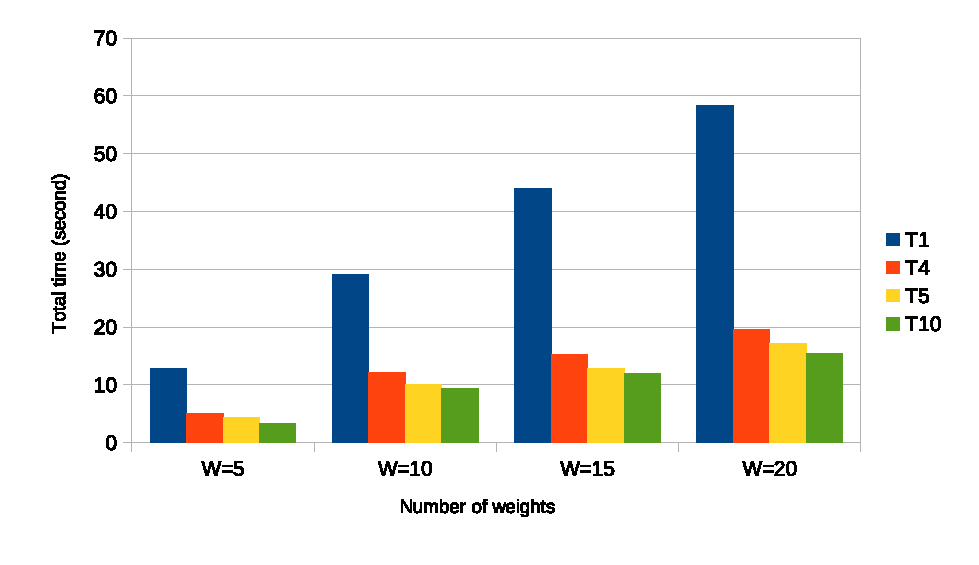
\includegraphics[scale=0.7]{time_comparison}
\par\end{centering}
\caption{Time comparison when the proposed method applied to Neural Network
training.\label{fig:Time-comparison}}
\end{figure}
\begin{table}
\caption{Experiments for the proposed method using different options for the
propagation method. The number of processing threads was set to 10.
Numbers in cells represent average function calls for every test function.\label{tab:propagation}}

\centering{}%
\begin{tabular}{>{\centering}p{0.19\textwidth}>{\centering}p{0.19\textwidth}>{\centering}p{0.19\textwidth}>{\centering}p{0.19\textwidth}>{\centering}p{0.19\textwidth}}
\hline 
\textbf{FUNCTION} & \textbf{1 to 1} & \textbf{1 to N} & \textbf{N to 1} & \textbf{N to N}\tabularnewline
\hline 
BF1 & 4887 & 4259 & 4209 & 2792\tabularnewline
\hline 
BF2 & 4577 & 4021 & 3917 & 2691\tabularnewline
\hline 
BRANIN & 3895 & 3378 & 3307 & 2382\tabularnewline
\hline 
CIGAR10 & 1875 & 1874 & 1871 & 1873\tabularnewline
\hline 
CM4 & 2243(0.97) & 2173 & 2136(0.97) & 2030\tabularnewline
\hline 
DISCUS10 & 1807 & 1810 & 1808 & 1809\tabularnewline
\hline 
EASOM & 1791 & 1790 & 1791 & 1789\tabularnewline
\hline 
ELP10 & 29944 & 42025 & 22876 & 19117\tabularnewline
\hline 
EXP4 & 1806 & 1807 & 1811 & 1806\tabularnewline
\hline 
EXP16 & 1830 & 1829 & 1828 & 1824\tabularnewline
\hline 
EXP64 & 1838 & 1838 & 1838 & 1836\tabularnewline
\hline 
GKLS250 & 1818 & 1812 & 1810 & 1802\tabularnewline
\hline 
GKLS350 & 2195 & 2163 & 2109 & 2011(0.97)\tabularnewline
\hline 
GRIEWANK2 & 4208 & 3620 & 3514 & 2445(0.80)\tabularnewline
\hline 
POTENTIAL3 & 5598 & 4445 & 4353 & 2521\tabularnewline
\hline 
POTENTIAL5 & 8620 & 7475 & 7025 & 3374\tabularnewline
\hline 
HANSEN & 9242 & 6075 & 6181 & 3135\tabularnewline
\hline 
HARTMAN3 & 2883 & 2664 & 2593 & 2207\tabularnewline
\hline 
HARTMAN6 & 4877(0.97) & 4327(0.83) & 4362(0.80) & 2834(0.57)\tabularnewline
\hline 
RASTRIGIN & 3707 & 3213 & 2870 & 2220(0.90)\tabularnewline
\hline 
ROSENBROCK4 & 9473 & 8294 & 7883 & 7084\tabularnewline
\hline 
ROSENBROCK8 & 20654 & 24470 & 15919 & 19272\tabularnewline
\hline 
SHEKEL5 & 5065(0.80) & 7556 & 5386(0.93) & 4456(0.70)\tabularnewline
\hline 
SHEKEL7 & 6996 & 7207(0.90) & 6488(0.93) & 4493(0.80)\tabularnewline
\hline 
SHEKEL10 & 7283 & 6812(0.93) & 6440 & 3916(0.73)\tabularnewline
\hline 
SINU4 & 4434 & 4204 & 4020 & 2796(0.97)\tabularnewline
\hline 
SINU8 & 4523 & 5386 & 4605 & 3341(0.90)\tabularnewline
\hline 
TEST2N4 & 6834 & 5777 & 5625 & 3609(0.97)\tabularnewline
\hline 
TEST2N5 & 8050 & 6695(0.97) & 6647 & 4179(0.73)\tabularnewline
\hline 
TEST2N6 & 9175 & 7770(0.93) & 7660 & 4522(0.53)\tabularnewline
\hline 
TEST2N7 & 9760 & 9259(0.77) & 9081 & 5200(0.57)\tabularnewline
\hline 
TEST30N3 & 2994 & 2814 & 2653 & 2210\tabularnewline
\hline 
TEST30N4 & 3031 & 2797 & 2700 & 2107\tabularnewline
\hline 
\textbf{AVERAGE} & \textbf{197913(0.99)} & \textbf{201649(0.98)} & \textbf{167316(0.98)} & \textbf{129683(0.91)}\tabularnewline
\hline 
\end{tabular}
\end{table}
\begin{table}
\caption{Compare the proposed method against other variants of the Differential
Evolution technique.\label{tab:deVariants}}

\centering{}%
\begin{tabular}{>{\centering}p{0.19\textwidth}>{\centering}p{0.19\textwidth}>{\centering}p{0.19\textwidth}>{\centering}p{0.19\textwidth}>{\centering}p{0.19\textwidth}}
\hline 
\textbf{FUNCTION} & \textbf{PROPOSED} & \textbf{ORIGINAL DE} & \textbf{DERL} & \textbf{DELB}\tabularnewline
\hline 
BF1 & 4887 & 5516 & 2881 & 5319\tabularnewline
\hline 
BF2 & 4577 & 5555 & 2895 & 5405\tabularnewline
\hline 
BRANIN & 3895 & 5656 & 2857 & 4830\tabularnewline
\hline 
CIGAR10 & 1875 & 88396 & 66161 & 58460\tabularnewline
\hline 
CM4 & 2243(0.97) & 9107 & 3856 & 6014\tabularnewline
\hline 
DISCUS10 & 1807 & 87657 & 55722 & 49014\tabularnewline
\hline 
EASOM & 1791 & 7879 & 7225 & 14934\tabularnewline
\hline 
ELP10 & 29944 & 33371 & 9345 & 39890\tabularnewline
\hline 
EXP4 & 1806 & 6027 & 2638 & 4142\tabularnewline
\hline 
EXP16 & 1830 & 26194 & 25117 & 11740\tabularnewline
\hline 
EXP64 & 1838 & 26497 & 27831 & 18346\tabularnewline
\hline 
GKLS250 & 1818 & 3800 & 1983 & 3706\tabularnewline
\hline 
GKLS350 & 2195 & 6206 & 2901 & 5027\tabularnewline
\hline 
GRIEWANK2 & 4208 & 6365 & 3325 & 6165\tabularnewline
\hline 
POTENTIAL3 & 5598 & 82933 & 111496 & 44592\tabularnewline
\hline 
POTENTIAL5 & 8620 & 24118 & 61694 & 46557\tabularnewline
\hline 
HANSEN & 9242 & 18470 & 7123 & 12212\tabularnewline
\hline 
HARTMAN3 & 2883 & 4655 & 2205 & 4124\tabularnewline
\hline 
HARTMAN6 & 4877(0.97) & 15488 & 5343 & 7215(0.93)\tabularnewline
\hline 
RASTRIGIN & 3707 & 6362 & 3102 & 5704\tabularnewline
\hline 
ROSENBROCK4 & 9473 & 16857 & 6679 & 10411\tabularnewline
\hline 
ROSENBROCK8 & 20654 & 56445 & 17198 & 22939\tabularnewline
\hline 
SHEKEL5 & 5065(0.80) & 13079 & 5224(0.90) & 8167\tabularnewline
\hline 
SHEKEL7 & 6996 & 12409 & 4994(0.97) & 8093\tabularnewline
\hline 
SHEKEL10 & 7283 & 13238 & 5240 & 8822\tabularnewline
\hline 
SINU4 & 4434 & 8977 & 3828 & 6052\tabularnewline
\hline 
SINU8 & 4523 & 28871 & 9318 & 10157\tabularnewline
\hline 
TEST2N4 & 6834 & 10764 & 4529 & 7331\tabularnewline
\hline 
TEST2N5 & 8050 & 15568 & 5917 & 8969\tabularnewline
\hline 
TEST2N6 & 9175 & 21185 & 7613 & 10648\tabularnewline
\hline 
TEST2N7 & 9760 & 28411 & 9492 & 12252\tabularnewline
\hline 
TEST30N3 & 2994 & 4965 & 2758 & 4693\tabularnewline
\hline 
TEST30N4 & 3031 & 5123 & 2688 & 5153\tabularnewline
\hline 
\textbf{AVERAGE} & \textbf{197913(0.99)} & \textbf{706144} & \textbf{491178(0.99)} & \textbf{477083(0.99)}\tabularnewline
\hline 
\end{tabular}
\end{table}
\begin{figure}
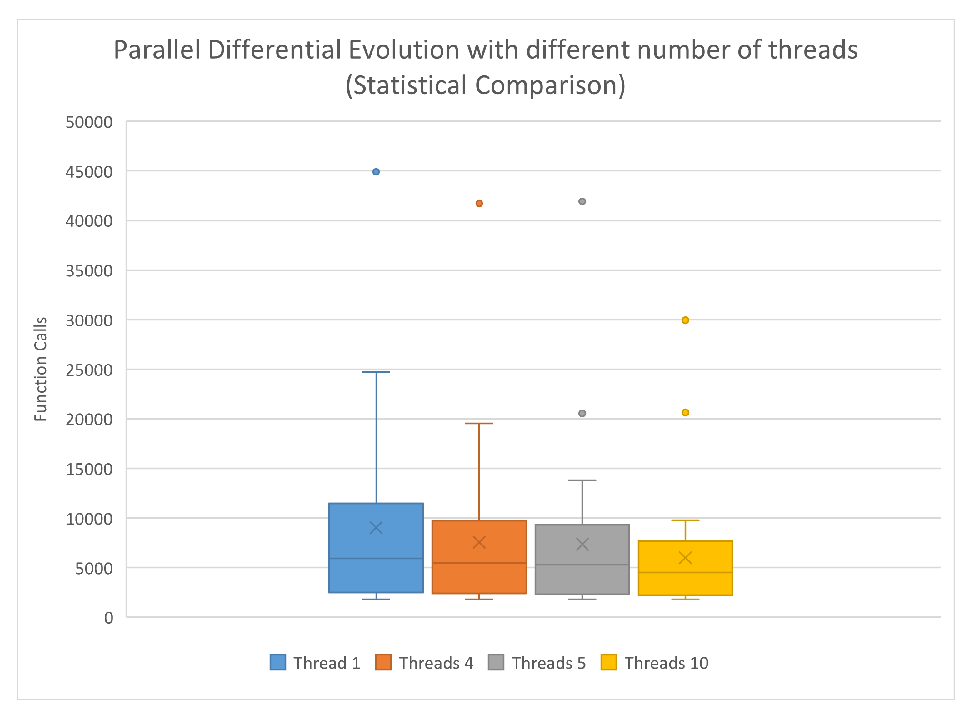
\includegraphics[scale=0.7]{boxPlotThreads}

\caption{Statistical comparison for the proposed method and different number
of threads.\label{fig:boxplotThreads}}

\end{figure}
\begin{figure}
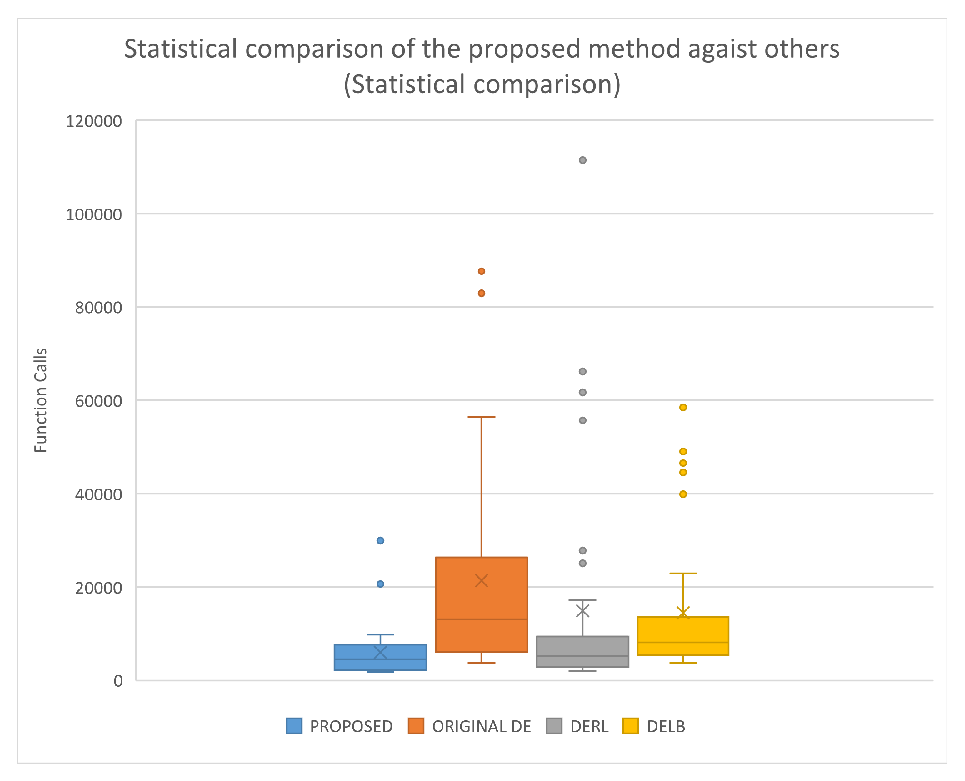
\includegraphics[scale=0.7]{boxPlotOthers}

\caption{Statistical comparison for the results of the proposed method against
different variations of the DE method.\label{fig:boxplotOthers}}

\end{figure}


\section{Conclusions\label{sec:Conclusions}}

A new global optimization technique was presented in this manuscript,
which can be performed in parallel computing environments. This method
is based on the well-known differential evolutionary technique and
partitions the initial population of agents, so as to create independent
populations that are executed on parallel computing units. The parallel
units periodically exchange the best values for the objective function
with each other, and from the experiments carried out it was found
that the most robust information exchange technique is the so-called
\textquotedbl 1 to 1\textquotedbl , where a randomly selected subpopulation
exchanges information with another randomly selected subpopulation.
Furthermore, a new termination method was proposed here which can
take full advantage of the parallel computing environment. With this
termination rule, the decision to terminate the method can be efficiently
made even by a small portion of the independent computing units.

From the experimental results, it appears that the proposed technique
can successfully find the global minimum in a series of problems from
the relevant literature, and in fact, as the number of parallel processing
units increases, the required number of function calls decreases.
Furthermore, after experiments on a difficult problem such as the
training of artificial neural networks, it was shown that the time
required for the optimization process decreases dramatically with
the increase of threads.

However, much can still be done to improve the methodology, such as
finding a better way of communication between parallel processing
units or even formulating more efficient termination criteria that
exploit parallel computing environments. In addition, the proposed
technique could be applied to other global optimization techniques
such as genetic algorithms or particle swarm optimization.

\vspace{6pt}


\authorcontributions{I.G.T. and V.C. conceived of the idea and methodology and supervised
the technical part regarding the software. I.G.T. conducted the experiments,
employing test functions, and provided the comparative experiments.
V.C. performed the statistical analysis and prepared the manuscript.
All authors have read and agreed to the published version of the manuscript.}

\funding{This research received no external funding.}

\institutionalreview{Not applicable.}

\informedconsent{Not applicable.}

\informedconsent{Not applicable.}

\acknowledgments{The experiments of this research work were performed at the high
performance computing system established at Knowledge and Intelligent
Computing Laboratory, Department of Informatics and Telecommunications,
University of Ioannina, acquired with the project “Educational Laboratory
equipment of TEI of Epirus” with MIS 5007094 funded by the Operational
Programme “Epirus” 2014--2020, by ERDF and national funds.}

\conflictsofinterest{The authors declare no conflict of interest.}

\sampleavailability{Not applicable.}

\appendixtitles{no}

\appendixstart{}

\begin{adjustwidth}{-\extralength}{0cm}{}


\reftitle{References}

\begin{thebibliography}{999}
\bibitem{go_physics1}M. Honda, Application of genetic algorithms
to modelings of fusion plasma physics, Computer Physics Communications
\textbf{231}, pp. 94-106, 2018.

\bibitem{go_physics2}X.L. Luo, J. Feng, H.H. Zhang, A genetic algorithm
for astroparticle physics studies, Computer Physics Communications
\textbf{250}, 106818, 2020.

\bibitem{go_physics3}T.M. Aljohani, A.F. Ebrahim, O. Mohammed, Single
and Multiobjective Optimal Reactive Power Dispatch Based on Hybrid
Artificial Physics--Particle Swarm Optimization, Energies \textbf{12},
2333, 2019.

\bibitem{go_chemistry1}P.M. Pardalos, D. Shalloway, G. Xue, Optimization
methods for computing global minima of nonconvex potential energy
functions, Journal of Global Optimization \textbf{4}, pp. 117-133,
1994.

\bibitem{go_chemistry2}A. Liwo, J. Lee, D.R. Ripoll, J. Pillardy,
H. A. Scheraga, Protein structure prediction by global optimization
of a potential energy function, Biophysics \textbf{96}, pp. 5482-5485,
1999.

\bibitem{go_chemistry3}J. An, G.He, F. Qin, R. Li, Z. Huang, A new
framework of global sensitivity analysis for the chemical kinetic
model using PSO-BPNN, Computers \& Chemical Engineering \textbf{112},
pp. 154-164, 2018.

\bibitem{go_econ1}Zwe-Lee Gaing, Particle swarm optimization to solving
the economic dispatch considering the generator constraints, IEEE
Transactions on \textbf{18} Power Systems, pp. 1187-1195, 2003.

\bibitem{go_econ2}M. Basu, A simulated annealing-based goal-attainment
method for economic emission load dispatch of fixed head hydrothermal
power systems, International Journal of Electrical Power \& Energy
Systems \textbf{27}, pp. 147-153, 2005.

\bibitem{go_med1}Y. Cherruault, Global optimization in biology and
medicine, Mathematical and Computer Modelling \textbf{20}, pp. 119-132,
1994.

\bibitem{go_med2}Eva K. Lee, Large-Scale Optimization-Based Classification
Models in Medicine and Biology, Annals of Biomedical Engineering \textbf{35},
pp 1095-1109, 2007.

\bibitem{crs1}W. L. Price, Global optimization by controlled random
search, Journal of Optimization Theory and Applications \textbf{40},
pp. 333-348, 1983.

\bibitem{crs2}Ivan Křivý, Josef Tvrdík, The controlled random search
algorithm in optimizing regression models, Computational Statistics
\& Data Analysis \textbf{20}, pp. 229-234, 1995.

\bibitem{crs3}M.M. Ali, A. Törn, and S. Viitanen, A Numerical Comparison
of Some Modified Controlled Random Search Algorithms, Journal of Global
Optimization \textbf{11},pp. 377--385,1997.

\bibitem{simann_major}S. Kirkpatrick, CD Gelatt, , MP Vecchi, Optimization
by simulated annealing, Science \textbf{220}, pp. 671-680, 1983.

\bibitem{simann1}L. Ingber, Very fast simulated re-annealing, Mathematical
and Computer Modelling \textbf{12}, pp. 967-973, 1989.

\bibitem{simann2}R.W. Eglese, Simulated annealing: A tool for operational
research, Simulated annealing: A tool for operational research \textbf{46},
pp. 271-281, 1990.

\bibitem{diffe1}R. Storn, K. Price, Differential Evolution - A Simple
and Efficient Heuristic for Global Optimization over Continuous Spaces,
Journal of Global Optimization \textbf{11}, pp. 341-359, 1997.

\bibitem{diffe2}J. Liu, J. Lampinen, A Fuzzy Adaptive Differential
Evolution Algorithm. Soft Comput \textbf{9}, pp.448--462, 2005.

\bibitem{pso_major}J. Kennedy and R. Eberhart, \textquotedbl Particle
swarm optimization,\textquotedbl{} Proceedings of ICNN'95 - International
Conference on Neural Networks, 1995, pp. 1942-1948 vol.4, doi: 10.1109/ICNN.1995.488968.

\bibitem{pso1}Riccardo Poli, James Kennedy kennedy, Tim Blackwell,
Particle swarm optimization An Overview, Swarm Intelligence \textbf{1},
pp 33-57, 2007. 

\bibitem{pso2}Ioan Cristian Trelea, The particle swarm optimization
algorithm: convergence analysis and parameter selection, Information
Processing Letters \textbf{85}, pp. 317-325, 2003.

\bibitem{aco1}M. Dorigo, M. Birattari and T. Stutzle, Ant colony
optimization, IEEE Computational Intelligence Magazine \textbf{1},
pp. 28-39, 2006.

\bibitem{aco2}K. Socha, M. Dorigo, Ant colony optimization for continuous
domains, European Journal of Operational Research 185, pp. 1155-1173,
2008.

\bibitem{ga1}D. Goldberg, Genetic Algorithms in Search, Optimization
and Machine Learning, Addison-Wesley Publishing Company, Reading,
Massachussets, 1989.

\bibitem{ga2}Z. Michaelewicz, Genetic Algorithms + Data Structures
= Evolution Programs. Springer - Verlag, Berlin, 1996.

\bibitem{ga3}S.A. Grady, M.Y. Hussaini, M.M. Abdullah, Placement
of wind turbines using genetic algorithms, Renewable Energy \textbf{30},
pp. 259-270, 2005.

\bibitem{go_review1}P.M. Pardalos, H.E. Romeijn, H. Tuy, Recent developments
and trends in global optimization, Journal of Computational and Applied
Mathematics \textbf{124}, pp. 209-228, 2000.

\bibitem{go_review2}D. Fouskakis, D. Draper, Stochastic Optimization:
a Review, International Statistical Review \textbf{70}, pp. 315-349,
2002.

\bibitem{de_app1}P. Rocca, G. Oliveri, A. Massa, Differential Evolution
as Applied to Electromagnetics, IEEE Antennas and Propagation Magazine.
\textbf{53}, pp. 38-49, 2011.

\bibitem{de_app2}W.S. Lee, Y.T. Chen, Y. Kao, Optimal chiller loading
by differential evolution algorithm for reducing energy consumption,
Energy and Buildings \textbf{43}, pp. 599-604, 2011.

\bibitem{de_app3}Y. Yuan, H. Xu, Flexible job shop scheduling using
hybrid differential evolution algorithms, Computers \& Industrial
Engineering \textbf{65}, pp. 246-260, 2013.

\bibitem{de_app4}L. Xu, H. Jia, C. Lang, X. Peng, K. Sun, A Novel
Method for Multilevel Color Image Segmentation Based on Dragonfly
Algorithm and Differential Evolution, IEEE Access \textbf{7}, pp.
19502-19538, 2019.

\bibitem{parallel-pso}J. F. Schutte, J. A. Reinbolt, B. J. Fregly, R.
T. Haftka, A. D. George, Parallel global optimization with the particle
swarm algorithm, International journal for Numerical methods in Engineering
\textbf{61}, pp. 2296-2315, 2004.

\bibitem{parallel-multistart}J. Larson and S.M. Wild, Asynchronously
parallel optimization solver for finding multiple minima, Mathematical
Programming Computation \textbf{10}, pp. 303-332, 2018.

\bibitem{parallel-doublepop}I.G. Tsoulos, A. Tzallas, D. Tsalikakis,
PDoublePop: An implementation of parallel genetic algorithm for function
optimization, Computer Physics Communications \textbf{209}, pp. 183-189,
2016.

\bibitem{msgpu1}R. Kamil, S. Reiji, An Efficient GPU Implementation
of a Multi-Start TSP Solver for Large Problem Instances, Proceedings
of the 14th Annual Conference Companion on Genetic and Evolutionary
Computation, pp. 1441-1442, 2012.

\bibitem{msgpu2}Van Luong T., Melab N., Talbi EG. (2011) GPU-Based
Multi-start Local Search Algorithms. In: Coello C.A.C. (eds) Learning
and Intelligent Optimization. LION 2011. Lecture Notes in Computer
Science, vol 6683. Springer, Berlin, Heidelberg. https://doi.org/10.1007/978-3-642-25566-3\_24

\bibitem{msgpu3}K. Barkalov, V. Gergel, Parallel global optimization
on GPU, J Glob Optim \textbf{66}, pp. 3--20, 2016. 

\bibitem{par_de1}M. Weber, F. Neri, V. Tirronen, Shuffle or update
parallel differential evolution for large-scale optimization, Soft
Comput \textbf{15}, pp. 2089--2107, 2011.

\bibitem{par_de2}Z. Chen, X. Jiang, J. Li, S. Li, L. Wang, PDECO:
Parallel differential evolution for clusters optimization, J. Comput.
Chem. \textbf{34}, pp. 1046-1059, 2013.

\bibitem{par_de3}D.R. Penas, J.R. Banga, P. Gonzalez, R. Doallo,
Enhanced parallel Differential Evolution algorithm for problems in
computational systems biology, Applied Soft Computing \textbf{33},
pp. 86-99, 2015.

\bibitem{par_de4}X. Sui , S.C. Chu, J.S. Pan, H.Luo, Parallel Compact
Differential Evolution for Optimization Applied to Image Segmentation,
Applied Sciences \textbf{10}, 2195, 2020.

\bibitem{de_island1}A. Skakovski, P. Jędrzejowicz, An island-based
differential evolution algorithm with the multi-size populations,
Expert Systems with Applications \textbf{126}, pp. 308-320, 2019.

\bibitem{de_island2}A. Skakovski and P. Jędrzejowicz, A Multisize
no Migration Island-Based Differential Evolution Algorithm With Removal
of Ineffective Islands, IEEE Access \textbf{10}, pp. 34539-34549,
2022.

\bibitem{de_main_paper}R. Storn, On the usage of differential evolution
for function optimization, In: Proceedings of North American Fuzzy
Information Processing, pp. 519-523, 1996.

\bibitem{compact_de0}F. Neri, E. Mininno, Memetic Compact Differential
Evolution for Cartesian Robot Control, IEEE Computational Intelligence
Magazine, \textbf{5}, pp. 54-65, 2010.

\bibitem{compact_de}E. Mininno, F. Neri, F. Cupertino and D. Naso,
Compact Differential Evolution, IEEE Transactions on Evolutionary
Computation \textbf{15}, pp. 32-54, 2011.

\bibitem{self_de}A. K. Qin, V. L. Huang and P. N. Suganthan, Differential
Evolution Algorithm With Strategy Adaptation for Global Numerical
Optimization, IEEE Transactions on Evolutionary Computation \textbf{13},
pp. 398-417, 2009.

\bibitem{fuzzy_de1}J. Liu, J. Lampinen, A Fuzzy Adaptive Differential
Evolution Algorithm, Soft Comput \textbf{9}, pp. 448--462, 2005.

\bibitem{fuzzy_de2}N. Hachicha, B. Jarboui, P. Siarry, A fuzzy logic
control using a differential evolution algorithm aimed at modelling
the financial market dynamics, Information Sciences \textbf{181},
pp. 79-91, 2011.

\bibitem{de_kaelo}P. Kaelo, M.M. Ali, A numerical study of some modified
differential evolution algorithms, European Journal of Operational
Research \textbf{169}, pp. 1176-1184, 2006.

\bibitem{island1}Arthur L. Corcoran, Roger L. Wainwright, A parallel
island model genetic algorithm for the multiprocessor scheduling problem,
SAC '94 Proceedings of the 1994 ACM symposium on Applied computing,
pp. 483-487, 1994.

\bibitem{island2}Darrell Whitley , Soraya Rana, Robert B. Heckendorn,
Island model genetic algorithms and linearly separable problems, Evolutionary
Computing Volume 1305 of the series Lecture Notes in Computer Science,
pp 109-125, 2005.

\bibitem{Powell}M.J.D Powell, A Tolerant Algorithm for Linearly Constrained
Optimization Calculations, Mathematical Programming \textbf{45}, pp.
547-566, 1989. 

\bibitem{Ali1}M. Montaz Ali, Charoenchai Khompatraporn, Zelda B.
Zabinsky, A Numerical Evaluation of Several Stochastic Algorithms
on Selected Continuous Global Optimization Test Problems, Journal
of Global Optimization \textbf{31}, pp 635-672, 2005. 

\bibitem{Floudas1}C.A. Floudas, P.M. Pardalos, C. Adjiman, W. Esposoto,
Z. G$\ddot{\mbox{u}}$m$\ddot{\mbox{u}}$s, S. Harding, J. Klepeis,
C. Meyer, C. Schweiger, Handbook of Test Problems in Local and Global
Optimization, Kluwer Academic Publishers, Dordrecht, 1999.

\bibitem{gkls}M. Gaviano, D.E. Ksasov, D. Lera, Y.D. Sergeyev, Software
for generation of classes of test functions with known local and global
minima for global optimization, ACM Trans. Math. Softw. \textbf{29},
pp. 469-480, 2003.

\bibitem{Jones}J.E. Lennard-Jones, On the Determination of Molecular
Fields, Proc. R. Soc. Lond. A \textbf{ 106}, pp. 463--477, 1924.

\bibitem{Sinu}Z.B. Zabinsky, D.L. Graesser, M.E. Tuttle, G.I. Kim,
Global optimization of composite laminates using improving hit and
run, In: Recent advances in global optimization, pp. 343-368, 1992.

\bibitem{openmp}R. Chandra, L. Dagum, D. Kohr, D. Maydan,J. McDonald
and R. Menon, Parallel Programming in OpenMP, Morgan Kaufmann Publishers
Inc., 2001.

\bibitem{newde}V. Charilogis , I.G. Tsoulos, A. Tzallas, E. Karvounis,
Modifications for the Differential Evolution Algorithm, Symmetry \textbf{14},
447, 2022.

\bibitem{ann-bishop}C.M. Bishop, Neural networks and their applications,
Review of Scientific Instruments \textbf{65}, pp. 1803-1832,1994.

\bibitem{wine1}M. Raymer, T.E. Doom, L.A. Kuhn, W.F. Punch, Knowledge
discovery in medical and biological datasets using a hybrid Bayes
classifier/evolutionary algorithm. IEEE transactions on systems, man,
and cybernetics. Part B, Cybernetics : a publication of the IEEE Systems,
Man, and Cybernetics Society, \textbf{33} , pp. 802-813, 2003.

\bibitem{wine2}P. Zhong, M. Fukushima, Regularized nonsmooth Newton
method for multi-class support vector machines, Optimization Methods
and Software \textbf{22}, pp. 225-236, 2007.
\end{thebibliography}

%%%%%%%%%%%%%%%%%%%%%%%%%%%%%%%%%%%%%%%%%%
%% for journal Sci
%\reviewreports{\\
%Reviewer 1 comments and authors' response\\
%Reviewer 2 comments and authors' response\\
%Reviewer 3 comments and authors' response
%}
%%%%%%%%%%%%%%%%%%%%%%%%%%%%%%%%%%%%%%%%%%

\end{adjustwidth}{}
\end{document}
